% =====================================================================
%  OMU-MAE  --  IEEE Intelligent Vehicles Symposium (IV) build
%  Class: IEEEtran (conference). Ships with Overleaf / TeX Live.
%  Page budget: IV is ~6 pages + references (confirm against the IV 2027
%  CFP; up to 2 extra pages are usually allowed for an over-length fee).
% =====================================================================
\documentclass[conference]{IEEEtran}
\IEEEoverridecommandlockouts

% ---- double-blind switch -------------------------------------------
% Named build for the defense / arXiv (\anonfalse, shows authors).
% For the double-blind IV submission set \anontrue ("Anonymous IV submission").
\newif\ifanon \anonfalse
% ---- optional figures (IV is ~6 pp: keep OFF to fit; ON for arXiv) --
\newif\ifextrafigs \extrafigsfalse
% --------------------------------------------------------------------

\usepackage{cite}
\usepackage{amsmath,amssymb,amsfonts}
\usepackage{graphicx}
\usepackage{booktabs}
\usepackage{array}
\usepackage{xcolor}
\usepackage{url}
\usepackage[hidelinks]{hyperref}
\usepackage{tikz}
\usetikzlibrary{positioning,arrows.meta,fit,backgrounds,calc}

\graphicspath{{figures/}}

\begin{document}

\title{OMU-MAE: Cross-Modal Masked Voxel Pretraining with\\
Frozen Vision Foundation Targets for Autonomous Driving Perception}

\ifanon
  \author{\IEEEauthorblockN{Anonymous IV submission}
  \IEEEauthorblockA{Paper ID XXXX}}
\else
  \author{%
  \IEEEauthorblockN{Badr Mellal, Rabab Benfouina, Ahmed Drissi el Maliani}
  \IEEEauthorblockA{LRIT Laboratory, Faculty of Sciences in Rabat\\
  Mohammed V University in Rabat, Morocco\\
  \texttt{badr\_mellal@um5.ac.ma, r.benfouina@um5r.ac.ma, a.elmaliani@um5r.ac.ma}}}
\fi

\maketitle

\begin{abstract}
We present OMU-MAE (\emph{Occupancy, Multi-modal, Unified} Masked
Autoencoder), a cross-modal voxel-level masked autoencoder for
self-supervised pretraining on paired camera and LiDAR data. Each scene
is voxelized into a $128\times128\times32$ grid at $0.4$\,m resolution;
per-voxel features are populated by projecting frozen DINOv2 ViT-B/14
patch features through the camera--LiDAR calibration. Following
Occupancy-MAE's range-aware schedule, 85\% of voxels are masked, and a
3D CNN encoder--decoder is trained to reconstruct both per-voxel
occupancy and the masked DINOv2 features. We pretrain on KITTI and
evaluate with a frozen-encoder linear probe on SemanticKITTI at
$1/5/10/100\%$ labels. Under an identical \emph{five-way} controlled
protocol, OMU-MAE attains $19.68\%$ mIoU at $100\%$ labels and wins at
every label fraction: $+14.19$\,pp over a random-init baseline,
$+1.77$\,pp over a faithful Occupancy-MAE re-implementation (isolating
the cross-modal target), $+3.27$\,pp over a no-mask
CleverDistiller-equivalent (isolating the masking inductive bias), and
$+4.22$\,pp over a re-implemented SLidR contrastive-distillation
baseline (masked reconstruction vs.\ contrastive distillation of the
\emph{same} frozen-VFM target). The full
pipeline pretrains in a few hours on a single GPU.
\ifanon
Code and pretrained weights will be released upon acceptance.
\else
Code and pretrained weights: \url{https://github.com/badrmellal/full_omu_mae}.
\fi

\end{abstract}

\begin{IEEEkeywords}
Self-supervised learning, masked autoencoders, autonomous driving,
LiDAR, multi-modal perception, vision foundation models, DINOv2,
3D semantic segmentation.
\end{IEEEkeywords}

\section{Introduction}

% Figure 1 teaser -- rendered PNG (always displays; regenerate via
% figures/make_teaser.py). Placed at the top of the Introduction (page 1).
\begin{figure*}[t]
\centering
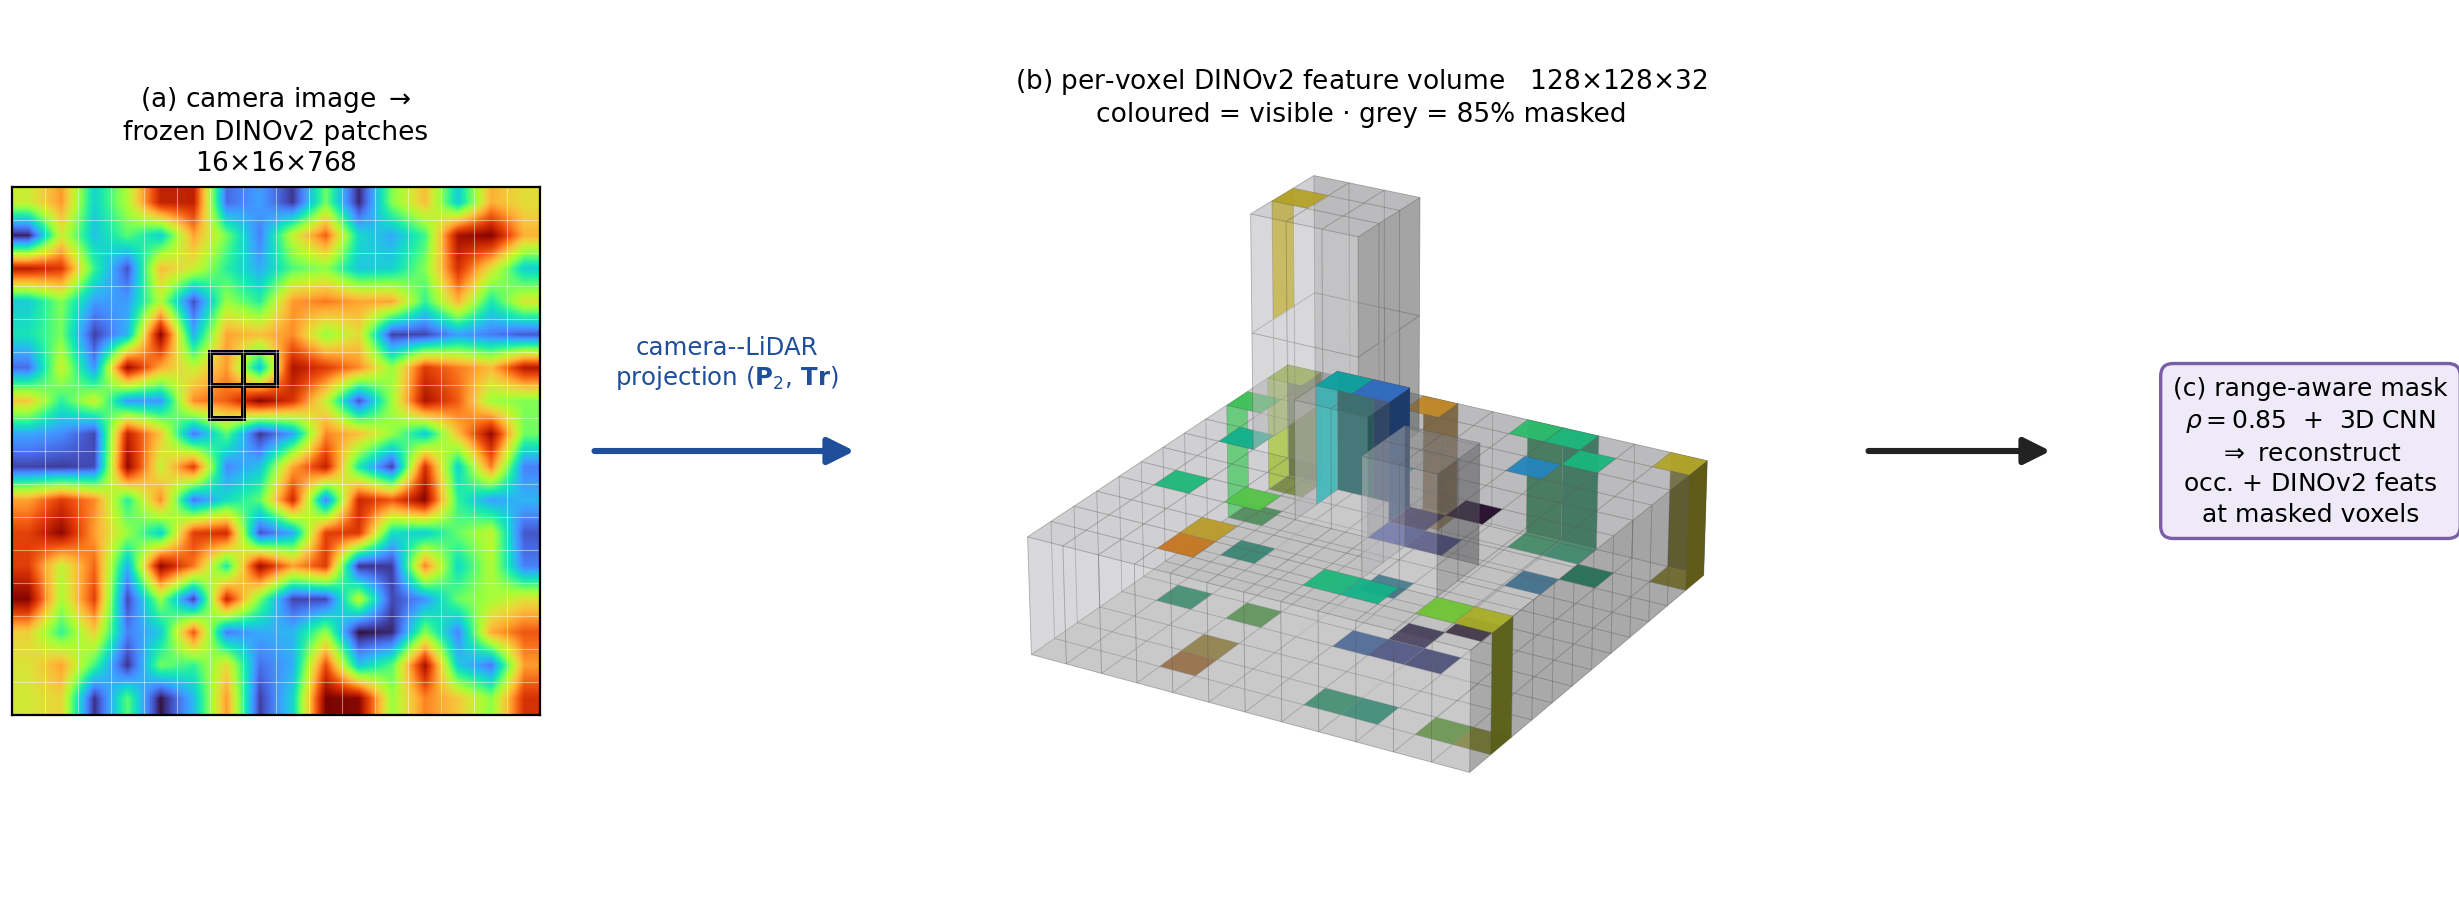
\includegraphics[width=0.97\textwidth]{teaser.png}
\caption{\textbf{OMU-MAE in one picture.} (a)~A frozen DINOv2 ViT-B/14 turns the
camera image into a $16{\times}16$ grid of $768$-d patch features. These are
projected through the camera--LiDAR calibration $(\mathbf{P}_2,\mathbf{Tr})$ to
(b)~populate a per-voxel feature volume aligned with the LiDAR occupancy grid
($0.4$\,m, $128{\times}128{\times}32$); $85\%$ of voxels are masked (grey),
$15\%$ stay visible (coloured). (c)~A 3D CNN reconstructs occupancy and the
DINOv2 features at the masked voxels. The target encoder is frozen, so this
$2\mathrm{D}\!\rightarrow\!3\mathrm{D}$ supervision cannot collapse to a trivial
solution.}
\label{fig:teaser}
\end{figure*}


Perception models for autonomous driving are still trained
predominantly with full supervision, and the supervision they need is
uncommonly expensive: annotating LiDAR for semantic segmentation means
assigning a class to every point of every scan, a slow, specialist task
that scales poorly with fleet data volumes~\cite{semantickitti}.
Self-supervised learning (SSL) offers the standard way out. In 2D
vision, three families of pretext tasks---contrastive instance
discrimination, self-distillation such as DINO and
DINOv2~\cite{dino,dinov2}, and masked autoencoding (MAE)~\cite{mae}---now
produce representations that match or exceed supervised pretraining,
transfer to downstream tasks from a handful of labels, and in the case
of DINOv2 yield dense per-patch features with strong emergent semantics
usable by a linear classifier alone. Bringing this label efficiency to
3D driving perception is the motivation for this work.

The transfer is not immediate, because driving scenes are inherently
multi-modal: they combine camera images dense in semantics with LiDAR
point clouds dense in geometry. A useful pretrained representation must
capture \emph{both}. This raises the problem we address: \emph{how to
pretrain a 3D encoder, without any human labels and on modest compute,
so that it absorbs the semantic richness of a 2D vision foundation
model (VFM) while retaining the spatial reasoning that 3D geometry
demands}. Two failure modes make this non-trivial. Methods that learn
both modality encoders jointly must fight representational collapse and
pay a heavy compute bill; methods that copy 2D features into 3D without
a spatial pretext task never force the encoder to reason about scene
structure at all.

Existing work sits on either side of this divide, and each side
inherits one of the two limitations. Multi-modal masked autoencoders
such as UniM\textsuperscript{2}AE~\cite{unim2ae} and
NS-MAE~\cite{nsmae} bring the MAE inductive bias to driving but
reconstruct \emph{raw} signals---pixels, points, or renderings---so the
model spends capacity on photometric and measurement nuisance rather
than semantics, and their jointly trained two-branch architectures are
compute-heavy. Distillation methods such as SLidR~\cite{slidr},
ScaLR~\cite{scalr} and CleverDistiller~\cite{cleverdistiller} instead
transfer \emph{frozen VFM features} to a LiDAR encoder---a
semantically strong, collapse-free target---but they distill at every
visible position, so nothing in the objective requires the encoder to
infer missing context from surrounding structure; the contrastive
variants further operate at sparse superpoint resolution, coarser than
the dense predictions downstream tasks need. What is missing is a
method that combines the strengths of the two families: the
\emph{semantic abstraction of a frozen VFM target} with the
\emph{context-inpainting inductive bias of masked reconstruction}.

OMU-MAE (\emph{Occupancy, Multi-modal, Unified} Masked Autoencoder)
occupies exactly this position. Each scene is voxelized on a dense
grid; frozen DINOv2 patch features are projected onto the voxels
through the camera--LiDAR calibration; 85\% of voxels are masked with
Occupancy-MAE's range-aware schedule~\cite{occmae}; and a 3D CNN
encoder--decoder reconstructs both binary occupancy and the DINOv2
features at masked positions. The two design choices are each doing
identifiable work. The \emph{frozen} target cannot co-adapt to the
predictor, which rules out the constant-output collapse mode of
joint-target prediction~\cite{ijepa,lejepa} by construction---no
regularization machinery needed---while still supplying dense semantic
supervision. \emph{Masked reconstruction} forces the encoder to inpaint
missing voxel context from surrounding visible voxels, an inductive
bias that distillation at every position does not impose. Whether that
bias actually improves downstream transfer is an empirical question,
and we answer it directly: we re-implement a contrastive (SLidR-style)
and a non-masked distillation (CleverDistiller-equivalent) baseline on
identical data, architecture and evaluation protocol, so the comparison
isolates the objective itself.

\paragraph{Contributions.}
\begin{enumerate}
\item OMU-MAE, a voxel-level masked autoencoder whose reconstruction
target combines binary occupancy with frozen DINOv2~\cite{dinov2}
features projected from the paired camera image; a dual loss, proposed
here, recovers both signals at masked positions.
\item A \emph{five-way} controlled study on KITTI / SemanticKITTI
(random init / Occupancy-MAE re-impl.\ / SLidR re-impl.\ / no-mask
CleverDistiller-equivalent / OMU-MAE) under one linear-probe protocol,
isolating each design choice: the cross-modal target is worth
$+1.77$\,pp over LiDAR-only masking, the masking bias $+3.27$\,pp over
non-masked distillation, and masked reconstruction $+4.22$\,pp over
contrastive distillation of the \emph{same} frozen-VFM target.
\item A deliberately lightweight recipe---dense voxel grid, single
3D CNN branch, no interaction module---that pretrains in a few hours on
one consumer GPU, with code and pretrained weights released.
\end{enumerate}

\section{Related Work}

\paragraph{Masked autoencoding for LiDAR.}
The MAE paradigm~\cite{mae} was extended to LiDAR by
Occupancy-MAE~\cite{occmae} and Voxel/LiDAR-MAE~\cite{hess2023lidar}, with
MAELi~\cite{maeli} scaling it to large sequences. Occupancy-MAE introduced
range-aware masking and reconstructs binary voxel occupancy. The proposed
OMU-MAE keeps its range-aware schedule but \emph{adds} a second target at
masked positions---a $768$-d vector matching the frozen DINOv2 patch
feature projected from the paired image. The joint dual objective
(occupancy plus frozen-feature reconstruction, both restricted to masked
positions) is proposed in this work; the occupancy term inherits
Occupancy-MAE's geometry supervision while the feature term injects
semantics that a binary target cannot carry. Regressing \emph{frozen}
teacher features at masked positions is well validated in 2D---MaskFeat's
ablations~\cite{maskfeat}, MILAN~\cite{milan} and EVA~\cite{eva} all show
it outperforms raw-pixel targets; OMU-MAE lifts this recipe to
cross-modal voxel-level driving scenes.

\paragraph{Multi-modal masked autoencoders.}
UniM\textsuperscript{2}AE~\cite{unim2ae} jointly trains both modality
encoders and reconstructs \emph{raw} pixels and LiDAR through a 3D
interaction module; NS-MAE~\cite{nsmae} reconstructs raw observations via
NeRF-style volumetric rendering. OMU-MAE differs on three axes, each with
a concrete payoff: the image encoder is \emph{frozen}, which removes the
collapse risk of joint training and halves the trainable footprint; the
cross-modal target is the frozen DINOv2 \emph{feature} volume rather than
raw pixels, so supervision carries semantics instead of photometric
nuisance; and there is no interaction module or back-projection---only
direct concatenation into the voxel input---which keeps the whole pipeline
a single 3D CNN branch that trains in a few hours on one GPU. The
trade-off is intentional: less expressive than a jointly trained
two-branch model, but far cheaper and collapse-free by construction.

\paragraph{Vision-foundation-model distillation to LiDAR.}
SLidR~\cite{slidr}, ScaLR~\cite{scalr} and SuperFlow++~\cite{superflow}
distill frozen-image features into LiDAR superpoints via InfoNCE at sparse
superpoint resolution; CleverDistiller~\cite{cleverdistiller} replaces
InfoNCE with a direct feature-similarity loss plus an occupancy auxiliary.
The frozen-VFM target $+$ occupancy task is shared with OMU-MAE; the
differentiator is \emph{masked reconstruction}. To make this comparison
concrete we re-implement both a contrastive (SLidR) and a no-mask
distillation (CleverDistiller-equivalent) variant inside our framework and
compare under an identical protocol (Sec.~\ref{sec:setup}).

\paragraph{JEPA and dense vision features.}
JEPA-family methods~\cite{ijepa,vjepa,lejepa,adljepa} predict latent
representations of masked targets, but their co-evolving target requires
careful regularization (VICReg~\cite{vicreg}) to avoid collapse; we
deliberately sidestep this with a frozen target. We use
DINOv2~\cite{dino,dinov2,dinov3} ViT-B/14 as that target for the quality of
its dense features and the public availability of weights via
\texttt{torch.hub}.

\section{Method}
\label{sec:method}

% Pipeline schematic (TikZ). Wrapped in \resizebox so it always fits the
% text width in both IEEEtran and the CVF/wacv two-column layout.
\begin{figure*}[t]
\centering
\resizebox{\textwidth}{!}{%
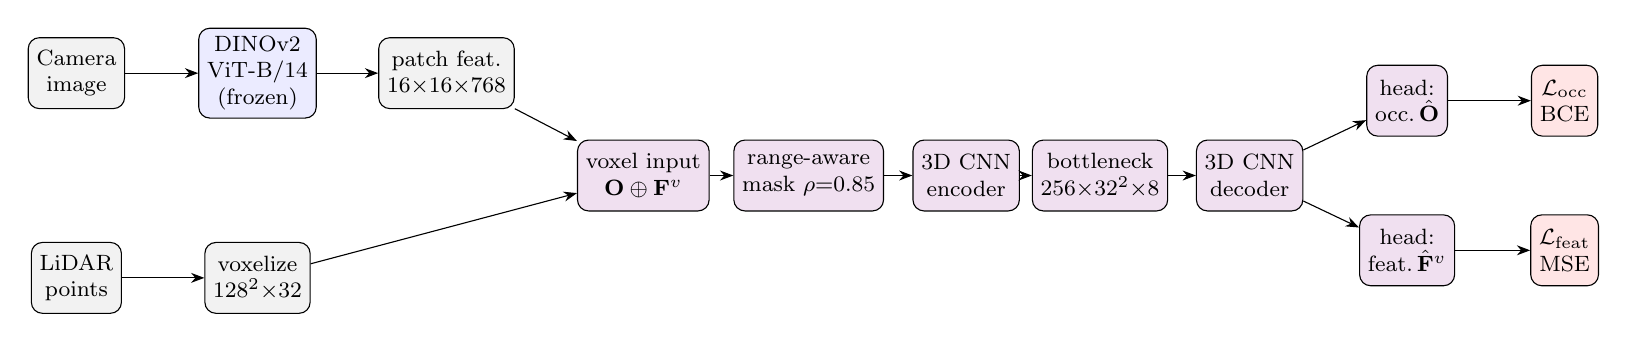
\begin{tikzpicture}[
  font=\footnotesize,
  >=Stealth,
  box/.style={draw, rounded corners, minimum height=9mm, align=center, inner sep=3pt},
  data/.style={box, fill=gray!10},
  frozen/.style={box, fill=blue!8},
  train/.style={box, fill=violet!12},
  loss/.style={box, fill=red!10}
]
% camera branch (top)
\node[data]   (img)   at (0,1.3)   {Camera\\image};
\node[frozen] (dino)  at (2.3,1.3)  {DINOv2\\ViT-B/14\\(frozen)};
\node[data]   (feat)  at (4.7,1.3)  {patch feat.\\$16{\times}16{\times}768$};
% lidar branch (bottom)
\node[data]   (lidar) at (0,-1.3)  {LiDAR\\points};
\node[data]   (vox)   at (2.3,-1.3) {voxelize\\$128^2{\times}32$};
% fused spine
\node[train]  (fuse)  at (7.2,0)   {voxel input\\$\mathbf{O}\oplus\mathbf{F}^v$};
\node[train]  (mask)  at (9.3,0)   {range-aware\\mask $\rho{=}0.85$};
\node[train]  (enc)   at (11.3,0)  {3D CNN\\encoder};
\node[train]  (bott)  at (13.0,0)  {bottleneck\\$256{\times}32^2{\times}8$};
\node[train]  (dec)   at (14.9,0)  {3D CNN\\decoder};
% heads + losses
\node[box,fill=violet!12] (occh) at (16.9,0.95) {head:\\occ.\,$\hat{\mathbf{O}}$};
\node[box,fill=violet!12] (fth)  at (16.9,-0.95) {head:\\feat.\,$\hat{\mathbf{F}}^v$};
\node[loss] (locc) at (18.9,0.95) {$\mathcal{L}_{\text{occ}}$\\BCE};
\node[loss] (lfeat) at (18.9,-0.95) {$\mathcal{L}_{\text{feat}}$\\MSE};
% arrows
\draw[->] (img)  -- (dino);
\draw[->] (dino) -- (feat);
\draw[->] (lidar)-- (vox);
\draw[->] (feat)  -- (fuse);
\draw[->] (vox)   -- (fuse);
\draw[->] (fuse) -- (mask);
\draw[->] (mask) -- (enc);
\draw[->] (enc)  -- (bott);
\draw[->] (bott) -- (dec);
\draw[->] (dec) -- (occh);
\draw[->] (dec) -- (fth);
\draw[->] (occh) -- (locc);
\draw[->] (fth)  -- (lfeat);
\end{tikzpicture}%
}
\caption{\textbf{OMU-MAE pretraining pipeline.} A paired RGB image (top)
is processed by a \emph{frozen} DINOv2 ViT-B/14 encoder; per-patch
features are projected via the camera--LiDAR calibration and
mean-aggregated per voxel. The LiDAR scan (bottom) is voxelized at
$0.4$\,m into a $128{\times}128{\times}32$ grid. The concatenated
cross-modal voxel input $\mathbf{O}\oplus\mathbf{F}^v$ is range-aware
masked ($\rho{=}0.85$), encoded by a 3D CNN, and decoded back to two
heads that reconstruct occupancy ($\mathcal{L}_{\text{occ}}$, BCE) and
DINOv2 features ($\mathcal{L}_{\text{feat}}$, MSE) at masked positions.}
\label{fig:pipeline}
\end{figure*}


Figure~\ref{fig:pipeline} gives the overall OMU-MAE pretraining pipeline.
The image branch feeds a frozen DINOv2 ViT-B/14 encoder, whose per-patch
features are projected through the camera--LiDAR calibration onto the
LiDAR voxel grid. The fused voxel input is masked, encoded by a 3D CNN,
and decoded back to two prediction heads, one for occupancy and one for
DINOv2 features, each evaluated at masked voxel positions only.

\subsection{Cross-modal voxel input}
For each scene we are given a paired RGB image
$\mathbf{I}\in\mathbb{R}^{3\times H\times W}$ and LiDAR point cloud
$\mathcal{P}=\{\mathbf{p}_i\in\mathbb{R}^4\}_{i=1}^{N}$ in the LiDAR
coordinate frame. KITTI calibration provides the projection matrices
$\mathbf{P}_2$ and $\mathbf{Tr}$ that take a LiDAR point into the
rectified left camera. We voxelize the scene over a fixed metric volume
centered on the ego-vehicle ($25.6\,\text{m}\times51.2\,\text{m}\times6.8\,\text{m}$)
at $0.4$\,m resolution, yielding a grid of size
$128\times128\times32$. Two voxel-level signals are computed:
\begin{itemize}
\item For occupancy, a binary tensor
$\mathbf{O}\in\{0,1\}^{X\times Y\times Z}$ marking voxels that contain at
least one LiDAR point.
\item For the cross-modal feature, a frozen DINOv2 ViT-B/14
encoder~\cite{dinov2} processes $\mathbf{I}$ at $224\times224$ resolution
to produce a $16\times16$ patch-feature grid
$\mathbf{F}\in\mathbb{R}^{16\times16\times768}$. For each LiDAR point we
project to image coordinates, identify the enclosing patch, and aggregate
(mean-pool) DINOv2 features into the corresponding voxel. The result is a
per-voxel feature volume $\mathbf{F}^v\in\mathbb{R}^{768\times X\times Y\times Z}$.
\end{itemize}
Voxels not visible from the camera (e.g.\ behind the vehicle, outside the
image FoV) receive zero features; this visibility mask is implicit in the
input and reproduced at decoding.

\subsection{Range-aware masking}
Following Occupancy-MAE~\cite{occmae}, voxels nearer the ego-vehicle
(where LiDAR is dense and semantic content is richest) are masked at a
higher rate. For voxel $(x,y,z)$ with metric distance $d$ from the
ego-origin we set the per-voxel mask probability
$\Pr[m_{xyz}{=}1]=\rho\cdot(1+\alpha d)^{-1}$ with global mask ratio
$\rho=0.85$ and decay $\alpha=0.5$. Both the occupancy and feature
channels are zeroed at masked locations and concatenated with a binary
mask indicator, giving an input tensor of shape
$(1+768+1)\times X\times Y\times Z$.

\subsection{Encoder, decoder architecture}
The encoder $g_\theta$ is a 4-stage 3D CNN (Conv3D $+$ GroupNorm $+$ GELU
blocks with strided downsampling) producing a bottleneck feature volume
$\mathbf{H}\in\mathbb{R}^{C\times X'\times Y'\times Z'}$ at $1/4$
resolution and $C=4\,d_{\text{feat}}=256$ channels, where
$d_{\text{feat}}=64$. The decoder mirrors the encoder via
trilinear-upsample $+$ Conv3D blocks. Two heads at the decoder output emit
(a)~a per-voxel occupancy logit and (b)~a per-voxel feature prediction in
$\mathbb{R}^{768}$.

\subsection{Dual reconstruction loss}
Let $\hat{\mathbf{O}}$ and $\hat{\mathbf{F}}^v$ denote the predicted
occupancy logits and features, and
$\mathcal{M}\in\{0,1\}^{X\times Y\times Z}$ the mask. We compute two
terms, each restricted to masked positions:
\begin{align}
\mathcal{L}_{\text{occ}} &= \frac{1}{|\mathcal{M}|}
\sum_{(x,y,z):\,m_{xyz}=1}\!\!\text{BCE}\!\left(\hat{O}_{xyz},O_{xyz}\right),\\
\mathcal{L}_{\text{feat}} &= \frac{1}{|\mathcal{M}\cap\mathcal{O}^+|}
\sum_{(x,y,z)\in\mathcal{M}\cap\mathcal{O}^+}\!\!\left\|\hat{\mathbf{F}}^v_{xyz}-\mathbf{F}^v_{xyz}\right\|_2^2,
\end{align}
where $\mathcal{O}^+=\{(x,y,z):O_{xyz}=1\}$ restricts the feature
reconstruction to \emph{occupied} voxels (predicting features for empty
space is uninformative). The combined objective is
$\mathcal{L}=\lambda_{\text{occ}}\mathcal{L}_{\text{occ}}+\lambda_{\text{feat}}\mathcal{L}_{\text{feat}}$
with $\lambda_{\text{occ}}=1.0$ and $\lambda_{\text{feat}}=0.5$. The
supervision targets are read from the un-masked voxel input (occupancy
$\mathbf{O}$ from the LiDAR voxelization, features $\mathbf{F}^v$ from the
frozen DINOv2 ViT); because the target encoder is frozen it cannot
co-adapt to the predictor, which rules out the trivial constant-output
collapse mode of joint-target prediction.

\section{Experimental Setup}
\label{sec:setup}

\paragraph{Pretraining data.}
We pretrain on KITTI odometry~\cite{kittiraw,kittibench}, which provides
paired left-camera images, Velodyne HDL-64E scans, and calibration. We
use all available frames (no subsampling) and voxelize each scene as in
Sec.~\ref{sec:method}.

\paragraph{Evaluation data.}
For evaluation we use SemanticKITTI~\cite{semantickitti}, which provides
per-point class labels. We follow the official train/validation split
(sequence~08 held out for validation), use the standard 19-class
evaluation mapping, voxelize each scan into the same
$128\times128\times32$ grid, and assign each voxel its majority label.
Voxels with no labeled points are marked \texttt{ignore}.

\paragraph{Linear-probe protocol.}
We evaluate the frozen pretrained encoder by attaching a single
$1\times1\times1$ 3D convolutional head ($C\!\rightarrow\!20$ classes) at
the bottleneck resolution and trilinearly upsampling logits to the full
grid. The encoder is frozen; only the head is trained. We train for $5$
epochs with AdamW, $\text{lr}=5\times10^{-4}$, cross-entropy with
\texttt{ignore\_index}$=0$, and sweep label fractions
$\{1\%,5\%,10\%,100\%\}$. This probes representation quality: any
non-trivial mIoU a linear head achieves must originate from features the
encoder already provides in linearly separable form.

\paragraph{Baselines (identical protocol).}
We compare four baselines against OMU-MAE under the \emph{same} 3D CNN
architecture and probe protocol; only the pretraining recipe differs.
\begin{itemize}
\item \textbf{Random init:} same architecture, freshly initialized
weights, no pretraining.
\item \textbf{Occupancy-MAE} (LiDAR-only re-impl.): truly LiDAR-only input
(occupancy $+$ mask indicator, no DINOv2 channels), range-aware masking
with the same schedule, focal BCE on masked occupancy only. Isolates the
contribution of the cross-modal DINOv2 target.
\item \textbf{SLidR} (contrastive re-impl.): a faithful in-framework
re-implementation of SLidR's~\cite{slidr} contrastive VFM distillation. We
compute SLIC superpixels on the image, mean-pool the frozen DINOv2
features per superpixel (the targets) and the encoder's voxel features per
corresponding superpoint, and train an InfoNCE loss between matched
superpixel/superpoint pairs. The student input is occupancy only (the VFM
features are the \emph{target}, not an input) and there is \emph{no}
masking. This isolates contrastive distillation vs.\ masked
reconstruction of the same frozen-VFM target.
\item \textbf{No-mask} (CleverDistiller-equivalent): OMU-MAE's
architecture and full cross-modal input, but with $\rho=0$ (no masking);
the model regresses occupancy and DINOv2 features at \emph{all} positions.
This is functionally equivalent to CleverDistiller's~\cite{cleverdistiller}
recipe (direct VFM feature regression $+$ occupancy auxiliary task) in our
voxel grid, and isolates the masking inductive bias.
\end{itemize}

\paragraph{Hyperparameters.}
Pretraining: AdamW, $\text{lr}=5\times10^{-4}$, weight decay $0.05$, batch
size $4$, $20{,}000$ steps, gradient clipping at norm $1.0$, mask ratio
$\rho=0.85$, range decay $\alpha=0.5$, $16{,}384$ LiDAR points per scene,
and a focal occupancy loss ($\alpha=0.25,\gamma=2.0$). The frozen target
is DINOv2 ViT-B/14 (768-d features). The architecture, training schedule,
probe protocol, and random seed are identical across all five conditions.
Pretraining runs on a single GPU (NVIDIA RTX PRO 6000); the full
five-variant pretraining plus probe sweep completes in well under a day.

\paragraph{Cross-sensor transfer (nuScenes).}
To test whether the learned representation transfers across LiDAR
sensors, scene compositions, and label vocabularies, we additionally
evaluate on nuScenes~\cite{nuscenes} (\texttt{v1.0-trainval}). We take
each KITTI-pretrained encoder \emph{frozen}, project LiDAR points into
whichever of the six surround cameras observes them, voxelize into the
same grid, train only a fresh linear probe on nuScenes labels at
$\{1\%,5\%,10\%,100\%\}$, and report mIoU on the official validation split
($6{,}019$ keyframes). This is a deliberately hard setting: a $64$-beam
KITTI encoder is transferred to a $32$-beam nuScenes sensor with a
different camera rig and class set, with no fine-tuning of the encoder. We
report a single seed; we discuss this as a limitation in
Sec.~\ref{sec:limitations}.

\section{Results}

% --- 5.1 is wrapped in \ifextrafigs: dropped automatically in the
%     ~6-page IEEE build, kept for the 8-page WACV / arXiv build. ---
\ifextrafigs
\subsection{Self-supervised pretraining dynamics}
\begin{figure*}[t]
\centering
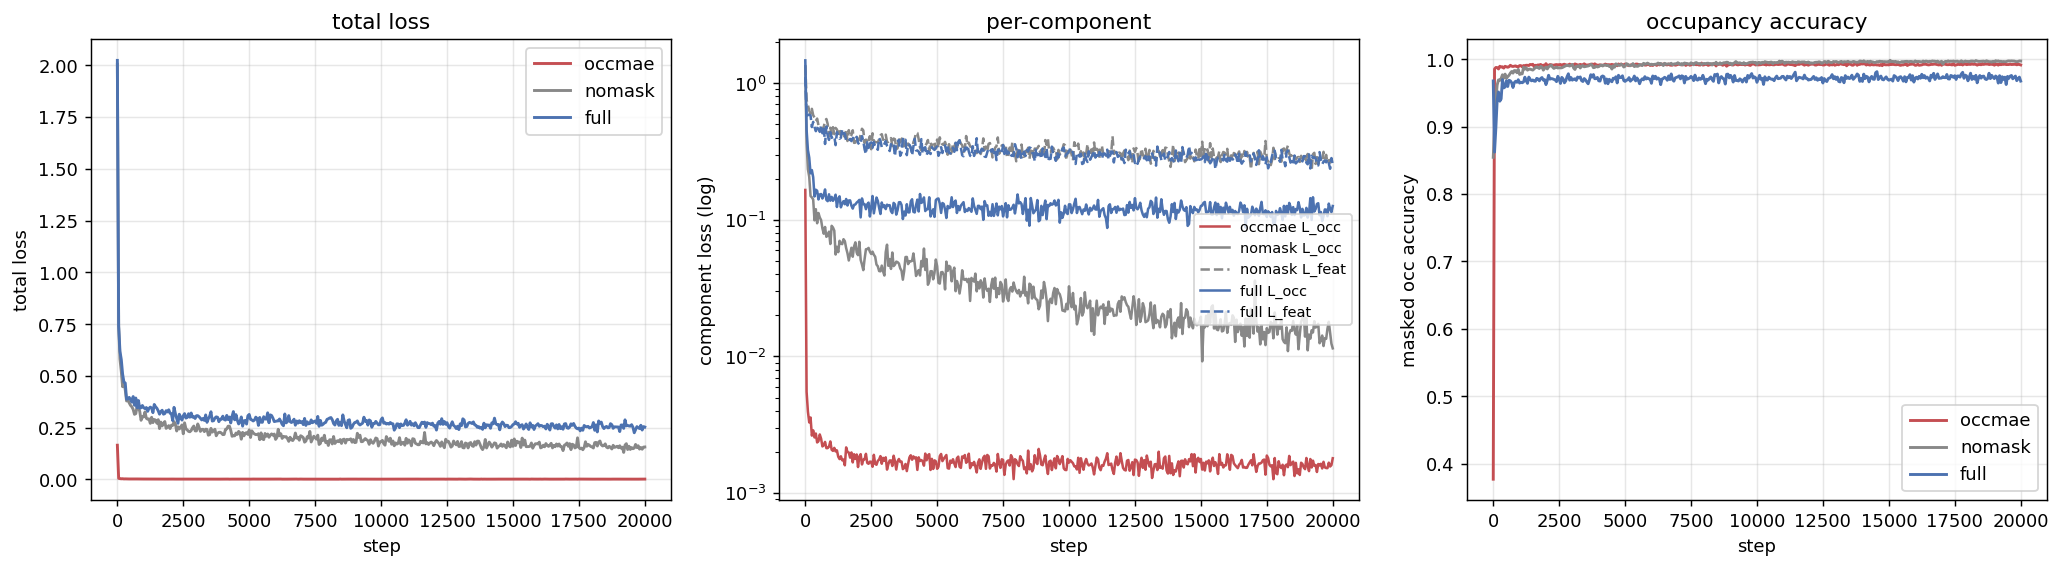
\includegraphics[width=\textwidth]{loss_curves.png}
\caption{\textbf{Pretraining dynamics.} Left: total loss vs.\ step.
Center: per-component decomposition (log-$y$) of
$\mathcal{L}_{\text{occ}}$ and $\mathcal{L}_{\text{feat}}$. Right:
masked-voxel occupancy accuracy. Total loss decreases steadily over the
$20$k pretraining steps; masked-voxel occupancy accuracy converges above
$97\%$ while the feature-reconstruction term decreases more gradually.}
\label{fig:dynamics}
\end{figure*}

Figure~\ref{fig:dynamics} shows the training-loss decomposition for the
OMU-MAE variants. Occupancy loss drops sharply early and the
masked-voxel occupancy accuracy saturates above $97\%$; the
feature-reconstruction term $\mathcal{L}_{\text{feat}}$ decreases more
gradually, consistent with the harder regression target.
Figure~\ref{fig:recon} shows a representative held-out scene: the input
camera image, ground-truth occupancy in bird's-eye view, the masking
pattern at $\rho=0.85$, and the model's predicted occupancy at masked
positions. The encoder recovers the dominant geometric structure despite
the high mask ratio.

\begin{figure*}[t]
\centering
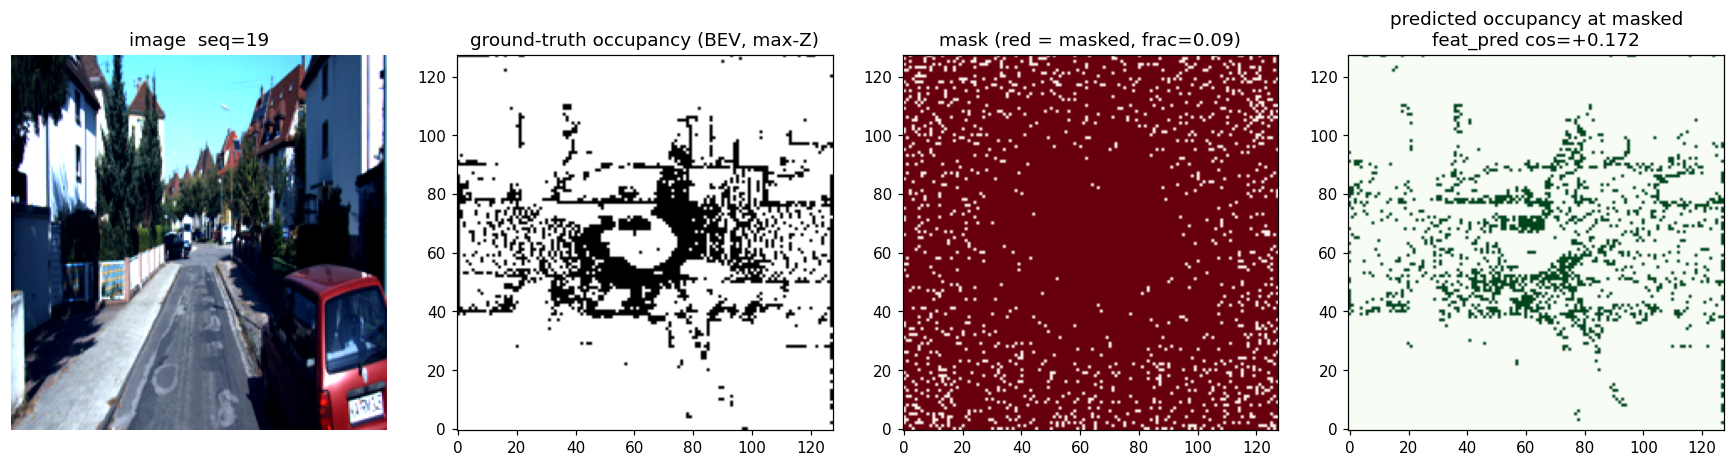
\includegraphics[width=\textwidth]{reconstruction_full.png}
\caption{\textbf{Reconstruction on a held-out scene (OMU-MAE).} Left to
right: input camera image, ground-truth voxel occupancy (BEV,
max-projected), masking pattern (masked voxels), and predicted occupancy
at masked positions.}
\label{fig:recon}
\end{figure*}
\fi

\subsection{Linear probe on SemanticKITTI}
\label{sec:probe}
Table~\ref{tab:probe} and Figure~\ref{fig:probe} report the headline
result. Under the identical five-way protocol, every pretraining variant
outperforms random initialization, and \textbf{OMU-MAE wins at every
label fraction}. Three controlled deltas isolate the design choices at
$100\%$ labels: OMU-MAE vs.\ Occupancy-MAE ($+1.77$\,pp) measures the
cross-modal DINOv2 target; OMU-MAE vs.\ the no-mask variant ($+3.27$\,pp)
measures the masking inductive bias; and OMU-MAE vs.\ the SLidR
re-implementation ($+4.22$\,pp) measures masked reconstruction against
contrastive distillation of the \emph{same} frozen-VFM target. All three
gains are consistent across the four label fractions.

\begin{table}[t]
\centering
\caption{\textbf{SemanticKITTI linear probe, five-way controlled
ablation.} mIoU (\%) over the 19 evaluation classes for the
frozen-encoder linear probe at four label fractions. All conditions use
the same dense 3D CNN architecture and probe protocol; only the
pretraining recipe differs. The last column gives the absolute gap (pp)
of OMU-MAE over each baseline at $100\%$ labels.}
\label{tab:probe}
\setlength{\tabcolsep}{4pt}
\begin{tabular}{lccccc}
\toprule
Pretraining variant & 1\% & 5\% & 10\% & 100\% & $\Delta$@100 \\
\midrule
Random init                                  & 4.95 & 5.72 & 6.14 & 5.50 & $-14.19$\\
Occupancy-MAE~\cite{occmae} (LiDAR-only)      & 13.88 & 16.34 & 17.08 & 17.91 & $-1.77$\\
SLidR~\cite{slidr} (contrastive re-impl.)     & 12.40 & 13.82 & 14.66 & 15.46 & $-4.22$\\
No-mask (CleverDist.-eq.)~\cite{cleverdistiller} & 9.75 & 12.26 & 14.18 & 16.41 & $-3.27$\\
\textbf{OMU-MAE (ours)} & \textbf{14.92} & \textbf{17.49} & \textbf{18.56} & \textbf{19.68} & --\\
\bottomrule
\end{tabular}
\end{table}

\begin{figure*}[t]
\centering
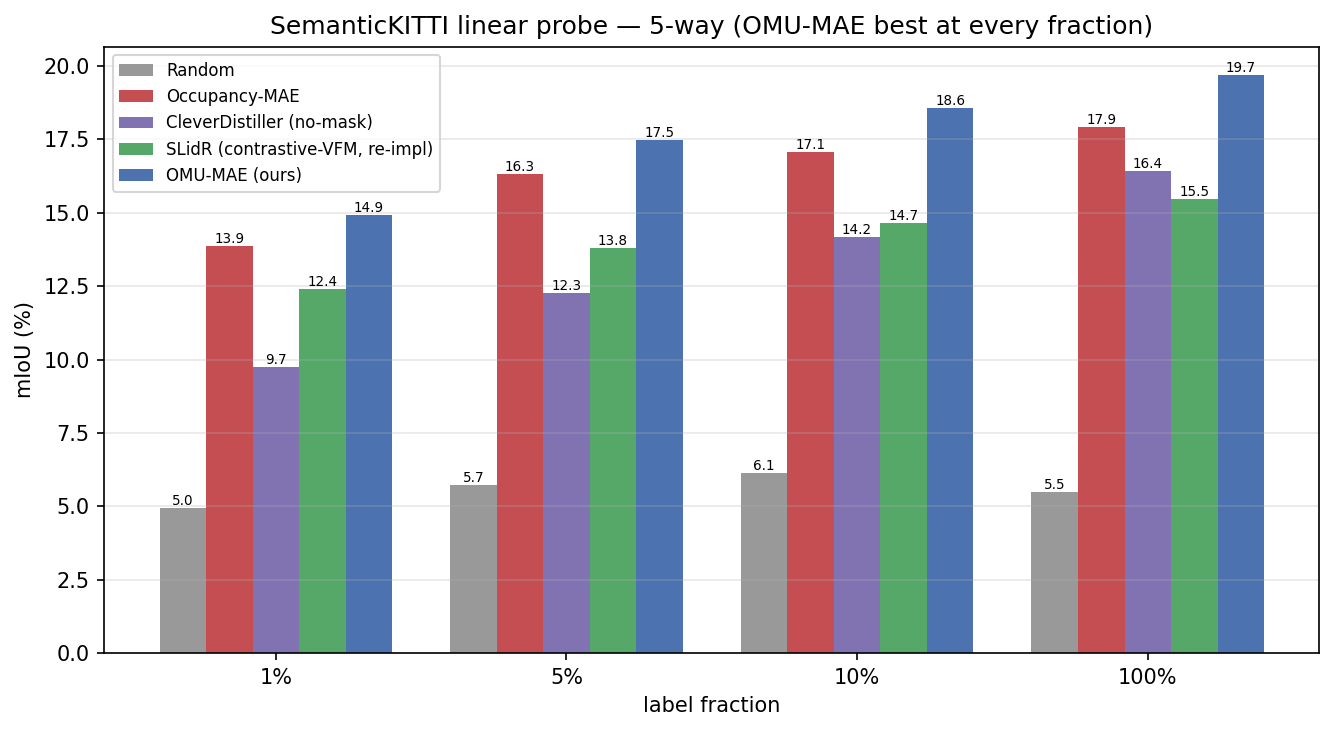
\includegraphics[width=\textwidth]{probe_comparison_5way.png}
\caption{\textbf{Linear-probe results (five-way).} Left: voxel mIoU on
SemanticKITTI validation across the four label fractions. Right: $\Delta$
in percentage points over random init at $100\%$ labels for each
pretrained variant.}
\label{fig:probe}
\end{figure*}

\paragraph{On the widening gap over random.}
OMU-MAE's gap over random init grows from $+9.97$\,pp at $1\%$ to
$+14.19$\,pp at $100\%$, which superficially contradicts the usual ``SSL
helps most when labels are scarce.'' We attribute this to
\emph{undertraining of the random baseline}: a freshly initialized 3D CNN
trained for $5$ probe epochs on a frozen, randomly projected feature space
has not converged, whereas the pretrained encoder already exposes
linearly separable structure that the probe reads off directly. A longer
probe schedule would partly close the random gap; we leave a probe-epoch
sweep to future work.

\subsection{Per-class analysis}
Figure~\ref{fig:perclass} reports per-class IoU at $100\%$ labels. The
OMU-MAE gains over random init concentrate on the dominant geometric and
semantic classes: building, sidewalk, road, car, terrain, vegetation,
fence and pole. Small or rare classes (motorcyclist, bicyclist, person,
bicycle, motorcycle) remain near-zero IoU under \emph{all} conditions. The
probe protocol, with $0.4$\,m voxelization that collapses small objects to
$1$--$2$ voxels and a single linear classifier, cannot recover their
fine-grained semantics regardless of the pretraining recipe.

\begin{figure*}[t]
\centering
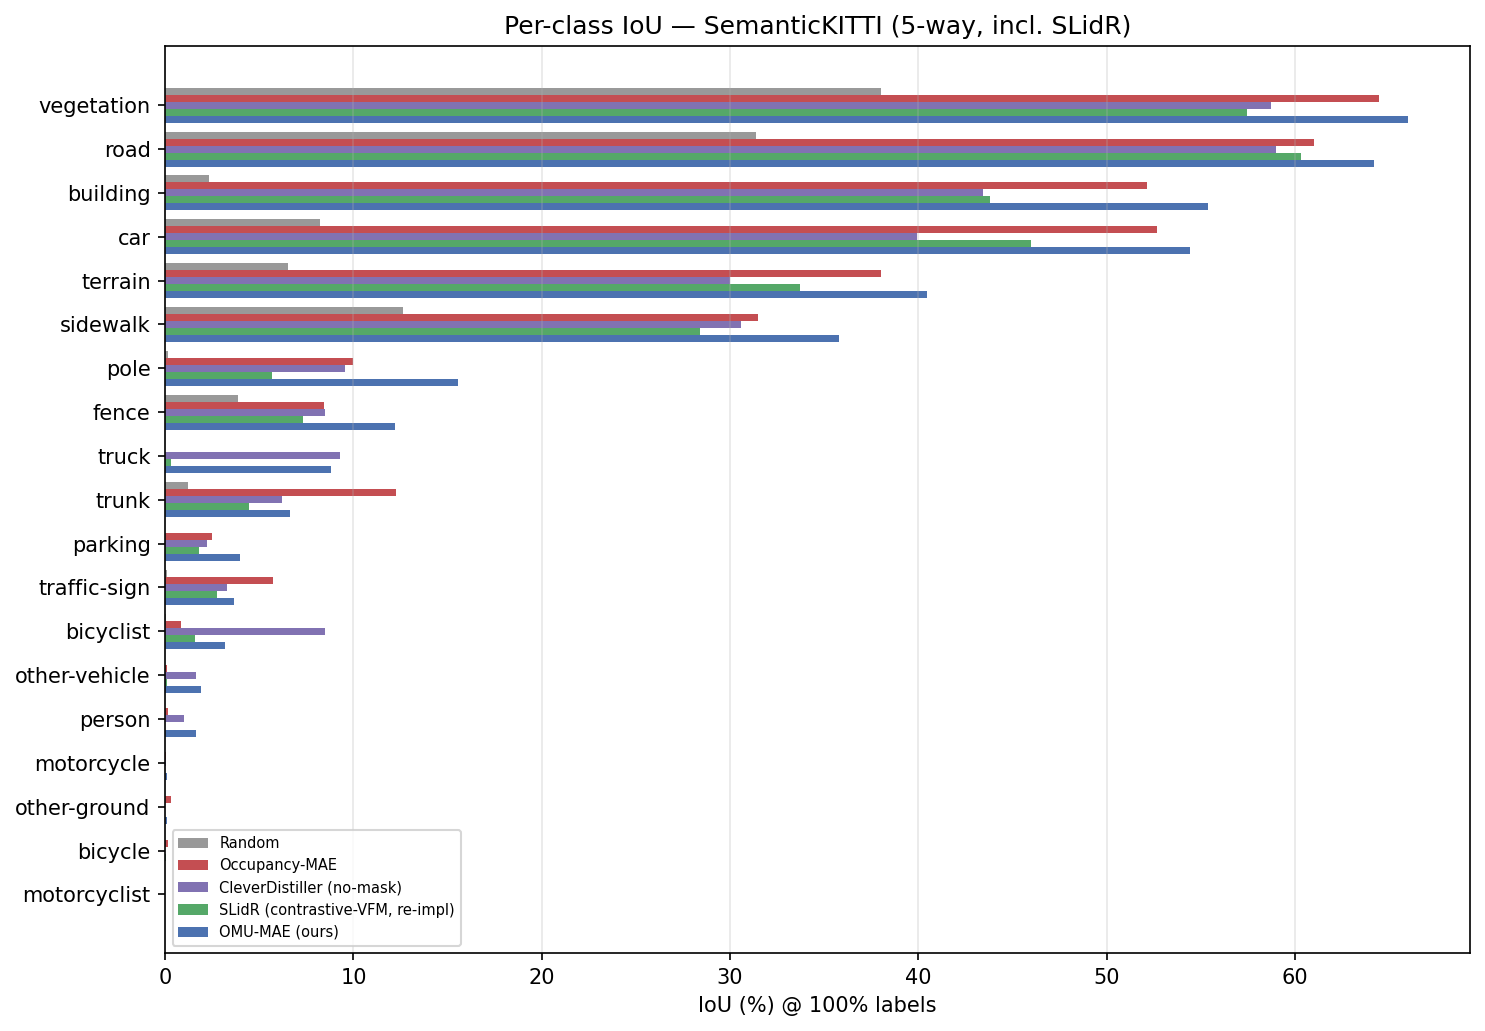
\includegraphics[width=\textwidth]{probe_per_class_5way.png}
\caption{\textbf{Per-class IoU at $100\%$ labels.} Left: per-class IoU
(\%); classes sorted by OMU-MAE IoU. Right: per-class $\Delta$ IoU (pp)
of OMU-MAE over random. Gains concentrate on geometric, semantic classes
(road, building, vegetation, terrain).}
\label{fig:perclass}
\end{figure*}

\subsection{Cross-sensor transfer to nuScenes}
\label{sec:nuscenes}
Table~\ref{tab:nusc} and Figure~\ref{fig:nusc} report the nuScenes
cross-sensor transfer. We report this result \emph{honestly}: absolute
mIoU is low for all variants ($<2.5\%$), reflecting how hard the setting
is---a $64$-beam KITTI encoder, frozen, probed on a $32$-beam nuScenes
sensor with a different camera rig and class vocabulary, single seed.
Because absolute mIoU is low and single-seed, we read the table
qualitatively rather than as a precise ranking. The robust pattern is that
the two cross-modal DINOv2-target variants---OMU-MAE and its no-mask
ablation---separate clearly from the LiDAR-only Occupancy-MAE, the
contrastive SLidR baseline, and random init at every fraction:
\emph{the frozen-VFM target, not the masking, is what carries across
sensors.} Within that DINOv2-target pair the masked and no-mask variants
are within run-to-run noise of each other. This is consistent with the
in-domain result rather than contradicting it: masking is the dominant
lever \emph{in domain}, while the cross-modal target---a core ingredient of
OMU-MAE shared with the no-mask ablation---is what generalizes
\emph{across sensors}. We do not over-claim a cross-sensor win for masking.

\begin{table}[t]
\centering
\caption{\textbf{nuScenes cross-sensor transfer} (frozen
KITTI-pretrained encoder, fresh linear probe, single seed, $6{,}019$
validation keyframes). mIoU (\%) at four label fractions; best per column
in bold. Both cross-modal DINOv2-target variants (OMU-MAE and its no-mask
ablation) separate from the LiDAR-only, contrastive, and random baselines:
the cross-modal target transfers, while masked-vs-no-mask is within
single-seed noise. Absolute mIoU is low---read qualitatively.}
\label{tab:nusc}
\setlength{\tabcolsep}{5pt}
\begin{tabular}{lcccc}
\toprule
Pretraining variant & 1\% & 5\% & 10\% & 100\% \\
\midrule
Random init                       & 0.45 & 0.58 & 0.68 & 0.83 \\
Occupancy-MAE~\cite{occmae}        & 0.30 & 0.37 & 0.46 & 0.61 \\
SLidR~\cite{slidr}                 & 0.28 & 0.60 & 0.74 & 0.94 \\
No-mask (CleverDist.-eq.)~\cite{cleverdistiller} & \textbf{1.06} & \textbf{1.54} & \textbf{1.71} & \textbf{2.45} \\
OMU-MAE (ours)                     & 0.76 & 1.41 & 1.49 & 1.62 \\
\bottomrule
\end{tabular}
\end{table}

\begin{figure}[t]
\centering
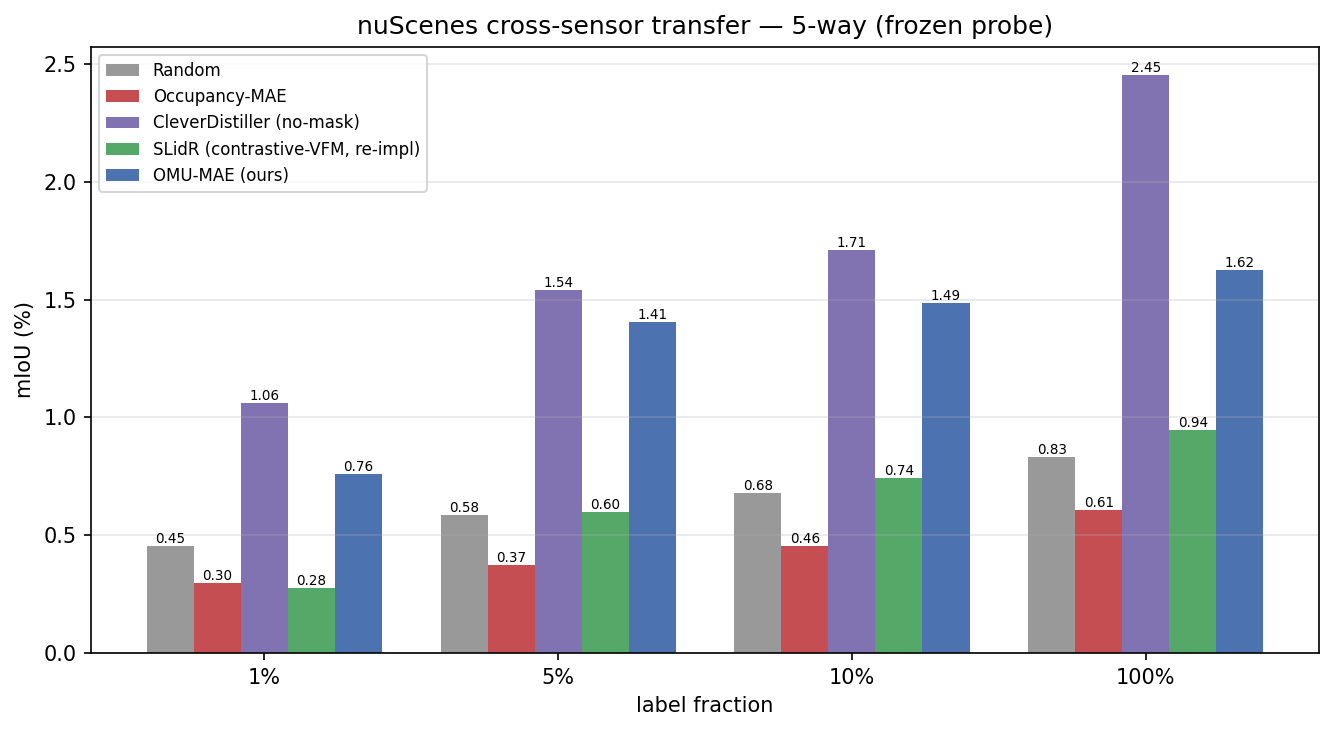
\includegraphics[width=\linewidth]{nuscenes_transfer_5way.png}
\caption{\textbf{nuScenes cross-sensor transfer (five-way).} Frozen
KITTI-pretrained encoder, fresh linear probe on nuScenes. Absolute mIoU is
low for all variants; the in-domain advantage of masking does not carry
across sensors.}
\label{fig:nusc}
\end{figure}

\subsection{Diagnostics}
\paragraph{Cross-modal scene retrieval.}
For completeness we report scene-level cross-modal retrieval: given the
scene-level mean encoder feature for one modality, retrieve the matching
scene from the other ($N=4{,}355$). Retrieval is essentially at chance
(image$\rightarrow$LiDAR Recall@1 $=0.02\%$ vs.\ chance $0.02\%$;
LiDAR$\rightarrow$image $0.05\%$; median rank $\approx N/2$). The per-voxel
cross-modal objective produces \emph{locally} useful features without by
itself inducing a globally aligned scene-level embedding; a scene-level
contrastive auxiliary or improved pooling would likely improve this, which
we leave to future work.

\section{Discussion}

\paragraph{Why masked reconstruction rather than contrastive distillation?}
The head-to-head against the SLidR re-implementation is the most direct
test of our central design choice. Both consume the \emph{same} frozen
DINOv2 target and differ only in objective---masked feature reconstruction
in a dense voxel grid vs.\ InfoNCE contrastive matching at sparse
superpoint resolution. OMU-MAE wins by $+2.52$ to $+4.22$\,pp, the gap
growing with labels. In our dense-voxel probe the SLidR baseline
($15.46\%$) even falls \emph{below} the LiDAR-only Occupancy-MAE
($17.91\%$): a dense per-voxel reconstruction target suits a dense voxel
encoder better than a sparse superpoint-level contrastive objective. We do
not read this as contrastive distillation being weak in general---SLidR
still beats random init by $+9.96$\,pp---but as evidence that the objective
should match the spatial granularity of the backbone.

\paragraph{Why a frozen DINOv2 target?}
A frozen target cannot co-adapt to the predictor, so the trivial
constant-output collapse mode that affects joint-target prediction
methods~\cite{ijepa,lejepa} cannot achieve low loss. This sidesteps the
regularization machinery (VICReg, LeJEPA, I-JEPA-style asymmetries) that an
evolving target requires, and lets a single consumer GPU train the pipeline
in a few hours.

\paragraph{On the non-obvious design choices.}
Most settings are standard and listed in Sec.~\ref{sec:setup}; three choices
are specific to this problem and worth motivating. \emph{Voxel resolution.}
$0.4$\,m is dictated by the cross-modal input: a $768$-d DINOv2 vector per
occupied voxel makes the dense feature volume grow cubically with
resolution, so $0.1$\,m reaches tens of gigabytes per scene and $0.2$\,m
already exhausts a single GPU; $0.4$\,m keeps the full five-variant pipeline
on one workstation GPU, at the cost of coarse small-object resolution
(Sec.~\ref{sec:limitations}). \emph{Masking.} The high ratio
($\rho{=}0.85$) follows MAE~\cite{mae} and Occupancy-MAE~\cite{occmae} and is
necessary because LiDAR voxel grids are highly redundant; range-aware
masking hides the dense near-field---where structure is learnable---more
than sparse far-field returns. \emph{Loss balancing.} The feature term is
down-weighted ($\lambda_{\text{feat}}{=}0.5$) so the hard $768$-d regression
does not overwhelm occupancy early in training, and a focal occupancy loss
counters the strong empty-vs-occupied imbalance. Architecture, schedule, and
seed are identical across all five conditions, so every reported difference
is attributable to the pretraining objective alone.

\section{Limitations and Future Work}
\label{sec:limitations}

We list the remaining limitations in roughly the order we believe they
should be addressed.

\paragraph{(1) Single seed.}
All numbers are from a single random seed; we report point estimates
without error bars. Our pretraining is seed-deterministic and the run is
resumable, so adding seeds is a matter of compute; a multi-seed study with
confidence intervals is the most important next step.

\paragraph{(2) Re-implementations, not original code.}
The Occupancy-MAE, SLidR and no-mask (CleverDistiller-equivalent)
baselines are faithful re-implementations inside our dense 3D CNN
framework, not the authors' original sparse-convolution code. They
preserve the scientifically relevant design choices (LiDAR-only input $+$
range-aware masking for Occupancy-MAE; SLIC-superpixel InfoNCE for SLidR;
all-position VFM regression $+$ occupancy auxiliary for CleverDistiller)
but differ in implementation details. Direct comparison against the
original codebases is future work. UniM\textsuperscript{2}AE~\cite{unim2ae}
(joint multi-modal MAE, raw-pixel target) and NS-MAE~\cite{nsmae}
(volumetric rendering) use a different training and evaluation protocol and
were not re-implemented.

\paragraph{(3) Single dataset.}
Our experiments are limited to KITTI / SemanticKITTI. Whether the gains
transfer across LiDAR sensors, scene compositions, and label vocabularies
(e.g.\ nuScenes or Waymo Open) is left to future work.

\paragraph{(4) End-to-end fine-tuning.}
We evaluate representation quality with the frozen linear probe, the
standard protocol for this purpose; the low-label-fraction probe results
($14.92\%$ mIoU at $1\%$ labels, $+9.97$\,pp over random) already speak to
label efficiency. Full end-to-end fine-tuning of the encoder---together
with a fine-tuned cross-sensor transfer---is a natural extension that we
leave to future work.

\paragraph{(5) Voxel resolution and probe depth.}
The $0.4$\,m grid is coarse for small classes (motorcycle, person,
bicyclist all $\sim 0$ mIoU under all conditions). A multi-resolution
variant or a sparse-voxel backbone~\cite{minkowski}, combined with a
shallow non-linear probe head, would likely improve fine-grained class
IoU without changing the SSL objective.

\section{Conclusion}

We presented OMU-MAE, a voxel-level masked autoencoder that uses frozen
DINOv2 features as the cross-modal reconstruction target. Under a five-way
controlled ablation on SemanticKITTI linear probing, OMU-MAE reaches
$19.68\%$ mIoU at $100\%$ labels and wins at every label fraction:
$+14.19$\,pp over random init, $+1.77$\,pp over a faithful Occupancy-MAE
re-implementation (the cross-modal target), $+3.27$\,pp over a no-mask
CleverDistiller-equivalent (the masking bias), and $+4.22$\,pp over a
re-implemented SLidR contrastive baseline (masked reconstruction vs.\
contrastive distillation of the same frozen-VFM target). A nuScenes
cross-sensor transfer study shows the representation carries some
sensor-agnostic signal---it beats random init, Occupancy-MAE and SLidR
out of domain---but the in-domain advantage of masking does not transfer,
a nuance we report honestly. Together with a preliminary negative result on
semantics-driven masking, these experiments isolate \emph{when} each
ingredient of cross-modal masked voxel pretraining helps, and when it does
not. The full pipeline trains in a few hours on a single GPU, and we
release code and pretrained weights to support reproduction.


\bibliographystyle{IEEEtran}
\bibliography{refs}

\end{document}
